\RequirePackage{fix-cm}
\documentclass[oneside, a4paper]{article}
\usepackage[a4paper,width=150mm,top=25mm,bottom=25mm,bindingoffset=6mm]{geometry}

% Required for inserting images
\usepackage{eso-pic,graphicx}
% misc
\usepackage{caption}
\DeclareCaptionType{equ}[][]
%\captionsetup[equ]{labelformat=empty}
\usepackage{subcaption}
\usepackage{multicol}
\usepackage{float}
\usepackage{adjustbox} % oversized table

% appendix
\usepackage[toc]{appendix}

% Default font to sans serif
\renewcommand{\familydefault}{\sfdefault}
\RequirePackage[T1]{fontenc} 
\RequirePackage[tt=false, type1=true]{libertine} 
\RequirePackage[varqu]{zi4} 
% \RequirePackage[libertine]{newtxmath}

% chapters and headers
\usepackage[Conny]{fncychap}

\usepackage{fancyhdr}
\pagestyle{fancy}
\renewcommand{\headrulewidth}{0.1pt}
% \renewcommand{\chaptermark}[1]{\markboth{\MakeUppercase{\textsf{{#1}}}}{}}
\renewcommand{\sectionmark}[1]{\markright{\MakeUppercase{\textsf{\thesection\ #1}}}{} }

% section styling
\usepackage{titlesec}

% algorithms
\usepackage{algorithm}
\usepackage{algpseudocode}

% theorems and definitions
\usepackage{amsthm}
\newtheorem{definition}{Definition}

% better tables
\usepackage{tabu}

% FAT FONTS
\usepackage{bm} % bold fonts in math mode
\newcommand\fat[1]{{\boldmath{\textbf{#1}}}}
\newcommand\emphasis[1]{{\scshape\bfseries#1}}

% mathematical fonts and graphics
\usepackage{mathtools}
\usepackage{xfrac} % sfrac for diagonal slashes in fractions
\usepackage{amsfonts} % math fonts
\usepackage{amssymb} % more math symbols (supsetneq etc.)
\usepackage{dbnsymb}
\usepackage{dsfont} % math fonts
\usepackage{bbm} % mathbb fonts
\usepackage{mathrsfs} % fancy swirly font
\usepackage{gensymb} % degree sign

% draw graphs
\usepackage[inline]{asymptote}
\usepackage{qtree}
\usepackage{tikz}
\usetikzlibrary{calc}

% nicer fractions
\usepackage{xfrac}
% cancel terms
\usepackage{cancel}

% units
\usepackage{siunitx}

% plots
\usepackage{pgfplots}
\usepackage{pgfplotstable}
\usepgfplotslibrary{external}
\usepgfplotslibrary{patchplots}
\usepgfplotslibrary{groupplots}
\pgfplotsset{compat=1.18} 
\tikzexternalize[prefix=tikz,optimize=false]

% define the Spectral_r color scheme
\usepackage[table, dvipsnames]{xcolor}
\definecolor{Spectral0}{RGB}{158, 1, 66}
\definecolor{Spectral1}{RGB}{213, 62, 79}
\definecolor{Spectral2}{RGB}{244, 109, 67}
\definecolor{Spectral3}{RGB}{253, 174, 97}
\definecolor{Spectral4}{RGB}{254,224,139}
\definecolor{Spectral5}{RGB}{255,255,191}
\definecolor{Spectral6}{RGB}{230,245,152}
\definecolor{Spectral7}{RGB}{171,221,164}
\definecolor{Spectral8}{RGB}{102,204,204}
\definecolor{Spectral9}{RGB}{50,136,189}
\definecolor{Spectral10}{RGB}{94,79,162}
\pgfplotsset{
  colormap={Spectral_r}{
    rgb255(0cm)=(94,79,162)         % 0.0
    rgb255(1cm)=(50,136,189)        % 0.1
    rgb255(2cm)=(102,204,204)       % 0.2
    rgb255(3cm)=(171,221,164)       % 0.3
    rgb255(4cm)=(230,245,152)       % 0.4
    rgb255(5cm)=(255,255,191)       % 0.5
    rgb255(6cm)=(254,224,139)       % 0.6
    rgb255(7cm)=(253,174,97)        % 0.7
    rgb255(8cm)=(244,109,67)        % 0.8
    rgb255(9cm)=(213,62,79)         % 0.9
    rgb255(10cm)=(158,1,66)         % 1.0
    }
}


% get width of given text
\usepackage{calc}

% define a horizontal spacer
\newcommand\horizontalspacer[0]{\vspace{5pt}\noindent\textcolor{lightgray}{\rule{\textwidth}{1mm}}
\vspace{5pt}}

% clickable links
\usepackage{hyperref}
\hypersetup{
    colorlinks,
    citecolor=black,
    filecolor=black,
    linkcolor=black,
    urlcolor=black
}
\renewcommand{\itemautorefname}{Item}
% fancy boxes
\usepackage{fancybox}
\newcommand{\equationnamed}[2]{%
  \setlength{\fboxsep}{2pt} % padding inside box
  \setlength{\fboxrule}{0.01pt}
  \begin{center}
    \begin{minipage}{\textwidth}
      \begin{center}\textsc{#1}\end{center}
      #2
    \end{minipage}
  \end{center}
}
\newcommand{\equationnamedbox}[2]{%
  \setlength{\fboxsep}{5pt} % padding inside box
  \setlength{\fboxrule}{0.01pt}
  \begin{center}
    \fbox{
      \begin{minipage}{\textwidth}
        \begin{center}\emphasis{#1}\end{center}
        #2
      \end{minipage}
    }
  \end{center}
}

% labels to enum items
\usepackage{enumitem}

\usepackage{array}

% make empty lines skip
% \usepackage{parskip}

% include pdfs 
\usepackage{pdfpages}

% code
\usepackage{minted}
\usepackage{listings}

% ~~~~~~~~~ TYPESETTING AND OTHER MACROS ~~~~~~~~~~~~~~~~~~~~~

\newenvironment{absolutelynopagebreak}
  {\par\nobreak\vfil\penalty0\vfilneg
   \vtop\bgroup}
  {\par\xdef\tpd{\the\prevdepth}\egroup
   \prevdepth=\tpd}

% ~~~~~~~~~ AFANCY CHAPTER HEADINGS ~~~~~~~~~~~~~~~~~~~~~~~~~~~
\makeatletter
\def\thickhrulefill{\leavevmode \leaders \hrule height 1ex \hfill \kern \z@}
\def\@makechapterhead#1{%
  %\vspace*{50\p@}%
  \vspace*{10\p@}%
  {\parindent \z@ \centering \reset@font
        \thickhrulefill\quad
        \scshape \@chapapp{} \thechapter
        \quad \thickhrulefill
        \par\nobreak
        \vspace*{10\p@}%
        \interlinepenalty\@M
        \hrule
        \vspace*{10\p@}%
        \Huge {\textbf{#1}} \par\nobreak
        \par
        \vspace*{10\p@}%
        \hrule
    \vskip 40\p@
    % \vskip 100\p@
  }}
\def\@makeschapterhead#1{%
  %\vspace*{50\p@}%
  \vspace*{10\p@}%
  {\parindent \z@ \centering \reset@font
        \thickhrulefill
        \par\nobreak
        \vspace*{10\p@}%
        \interlinepenalty\@M
        \hrule
        \vspace*{10\p@}%
        \Huge \bfseries #1\par\nobreak
        \par
        \vspace*{10\p@}%
        \hrule
    \vskip 40\p@
    % \vskip 100\p@
  }}

  \newcommand*{\@rowstyle}{}
  \newcommand*{\rowstyle}[1]{% sets the style of the next row
    \gdef\@rowstyle{#1}%
    \@rowstyle\ignorespaces%
  }
  \newcolumntype{=}{% resets the row style
    >{\gdef\@rowstyle{}}%
  }
  \newcolumntype{+}{% adds the current row style to the next column
    >{\@rowstyle}%
  }
  
\usepackage[pdftex,outline]{contour}

% ~~~~~~~~~ MATH MACROS ~~~~~~~~~~~~~~~~~~~~~~~~~~~~~~~~~~~~~~

% abs value macro
% \DeclarePairedDelimiter\abs{\lvert}{\rvert}
\newcommand\abs[1]{\left|#1\right|}
\newcommand\abss[1]{\left|\left|#1\right|\right|}
\newcommand\norm[1]{\left\lVert#1\right\rVert}
\newcommand\angled[1]{\left\langle#1\right\rangle}
\newcommand\round[1]{\left\lfloor#1\right\rceil}

\newcommand\dist[1]{\left|\left|#1\right|\right|}
\newcommand\arr[1]{\left\langle#1\right\rangle}
\newcommand\pdpi[0]{\frac{\partial}{\partial p_i}}

% define the laplace operator 
\newcommand*\Laplace{\mathop{}\!\mathbin\nabla^2}
\newcommand\vek[1]{\vec{\bm{#1}}}
\newcommand\nvek[1]{\hat{\vec{\bm{#1}}}}
\newcommand\mat[1]{{\mathds{#1}}}
\newcommand\br[1]{\left(#1\right)}

\DeclareMathOperator{\sgn}{sgn}
\DeclareMathOperator{\erf}{erf}

\DeclareMathOperator*{\argmax}{\arg\!\max}
\DeclareMathOperator*{\argmin}{\arg\!\min}

\newcommand\divergence{{\nabla\cdot}}

% ~~~~~~~~~~ HIGHLIGHT BLOCK ~~~~~~~~~~~~~~~~~~~~~~~~~~~~~~~~~~
\usepackage{mdframed}
\newmdenv[
  leftline=true,
  topline=false,
  rightline=false,
  bottomline=false,
  linecolor=gray!80,
  linewidth=1pt,
  innerleftmargin=10pt,
  innerrightmargin=0pt,
  innertopmargin=0pt,
  innerbottommargin=0pt,
  skipabove=\baselineskip,
  skipbelow=\baselineskip,
  backgroundcolor=white
]{highlightblock}

% ~~~~~~~~~ BIBLIOGRAPHY ~~~~~~~~~~~~~~~~~~~~~~~~~~~~~~~~~~~~~~

\usepackage[
  backend=biber,
  sorting=none,
  style=ieee,
  doi=false,
  % isbn=false,
  url=false,
  eprint=false
]{biblatex}
\addbibresource{refs.bib}

% ~~~~~~~~~ START ~~~~~~~~~~~~~~~~~~~~~~~~~~~~~~~~~~~~~~~~~~~~~~

\author{Julian Karrer}
\title{Metropolis Sampling}

\usepackage{transparent} % make background image semitransparent
\usepackage{ragged2e} % left flush env

\captionsetup[figure]{font=footnotesize,labelfont=footnotesize,justification=centering}
\setcounter{section}{0} 
\begin{document}

\begin{titlepage}
  \pagestyle{empty}
  \AddToShipoutPicture{%
  \AtPageLowerLeft{%
    \put(\dimexpr 0.5\paperwidth-0.45\paperwidth - 7cm\relax, %
         \dimexpr 0.5\paperheight-0.45\paperheight + 3cm\relax) %
    {%
      \transparent{0.04}%
      
\includegraphics[width=\paperwidth]{images/uni-siegel.pdf}%
    }%
  }%
}
  \begingroup
  \vspace*{6cm}
  \begin{FlushLeft}
    % \noindent %
    % \Large\textbf{Master's Project}\\
    \vspace{0.5cm}
    \noindent %
    \Huge\textbf{Metropolis Sampling}\\
    \Large{Seminar Report: Advanced Topics in Rendering}\\
    \vspace{0.5cm}
    \noindent %
    \Large{Julian Karrer}
  \end{FlushLeft}
  % \vspace{17cm}
  \vfill
  \begin{center}
    \large
    Faculty of Engineering\\
    Department of Computer Science\\
    Prof. Dr.-Ing. Matthias Teschner\\
    \vspace{0.1cm}
    \includegraphics*[width=5cm]{images/ufr-logo.png}
  \end{center}
  \endgroup
\end{titlepage}
% \captionsetup[figure]{font=normalsize,labelfont=normalsize}
\newpage{}
% \thispagestyle {empty}
\ClearShipoutPicture

\tableofcontents
\newpage

\section{Introduction}

The Metropolis-Hastings algorithm is one of the single most important algorithms in the history of Computer Science, with the editors of \textit{Computing in Science and Engineering} listing the algorithm among the ten most influential algorithms of the twentieth century \autocite{top10}. Despite its fame and groundbreaking contribution to the simulation of stochastic processes, its premise is rather simple: given any function $f: \Omega \to \mathds{R}^+$ from a measurable space $\Omega$ to non-negative real numbers $\mathds{R}^+$, generate a sequence of values $\vec{x}_1,\dots,\vec{x}_N$ that for large $N$ follow a distribution $p \propto f$. Solving this problem gives a general tool for various applications involving many-body systems, nondeterministic processes or the sampling of high-dimensional spaces \autocite{top10} and the algorithm is used in statistics, physics, economics and many other fields \autocite{survey}.

It is especially noteworthy that the algorithm makes close to no assumptions on the function being sampled: it can be of arbitrary dimensionality, there are no smoothness or continuity constraints, and it is therefore particularly suited to Monte Carlo light transport simulation in Computer Graphics, where an extremely high-dimensional path space with discontinuous occlusions is stochastically sampled to generate photorealistic images. This application of Metropolis sampling to rendering was popularized in the seminal work of \autocite[Veach and Guibas]{veach-guibas-mlt} on Metropolis Light Transport, which is highly relevant to this day. The Metropolis-Hastings algorithm has spawned an entire class of light transport algorithms called Markov Chain Monte Carlo or MCMC light transport \autocite{survey}. One of these applications is the Primary Sample Space Metropolis Light Transport or PSSMLT method, which will be discussed later in this report. An example of a multidimensional, discontinuous function being sampled using the Metropolis-Hastings algorithm is shown in \autoref{fig:title-image}.\\

In the following, the algorithm will be outlined, sufficient conditions for correct convergence will be given, the proposal distribution will be analysed and benefits and drawbacks of Metropolis-sampling will be outlined, before an application to rendering in the form of PSSMLT will be shown.


\begin{figure}
    \centering
    \begin{subfigure}[t]{0.5\textwidth}
        
\includegraphics[width=\textwidth]{./images/cover_smooth.png}
    \end{subfigure}%
    \begin{subfigure}[t]{0.5\textwidth}
        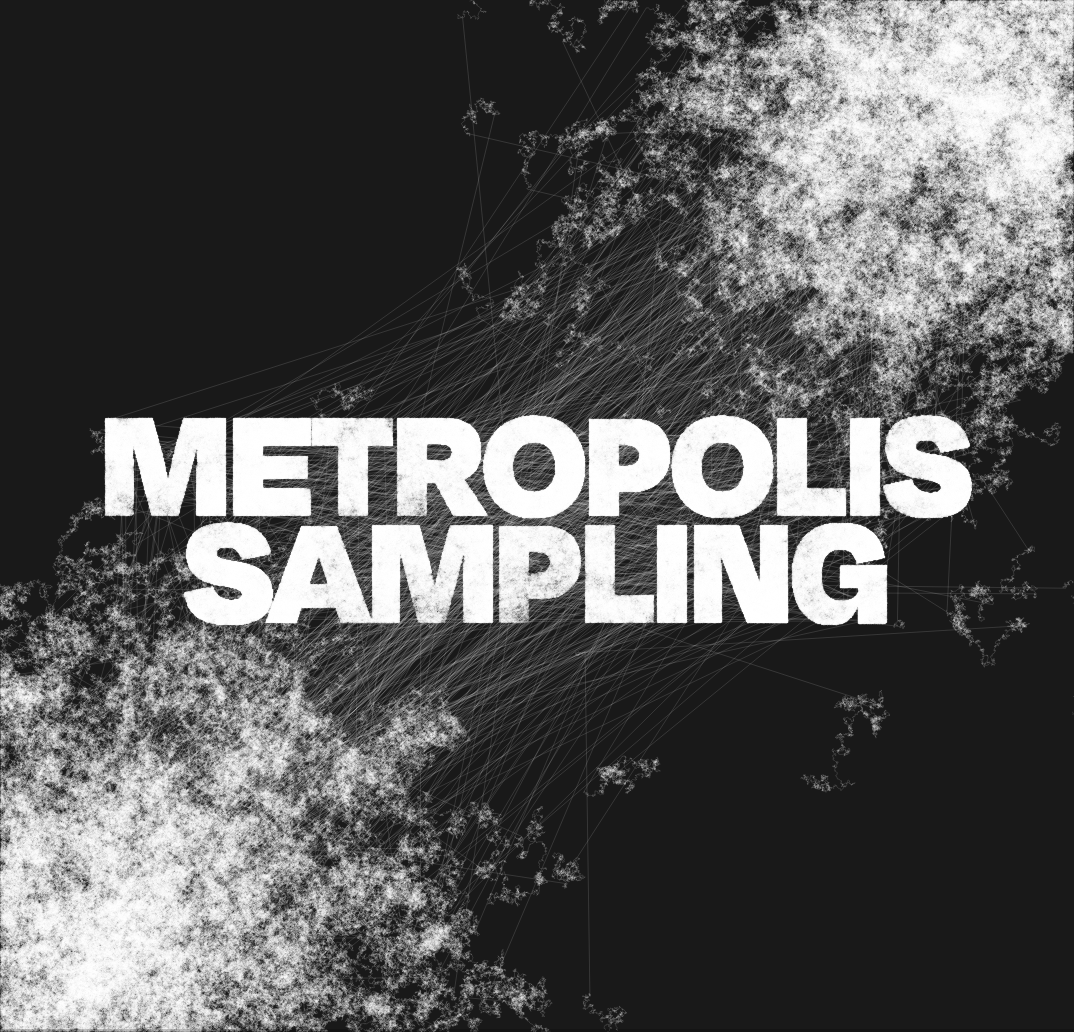
\includegraphics[width=\textwidth]{./images/cover_sampled.png}
    \end{subfigure}
    \caption{A two-dimensional function is illustrated in the left image, where brightness in the image is proportional to some function value $f(x,y)$. The function has booth smooth features, such as the Gaussian distributions in the corners, as well as a discontinuities at the letters spelling 'Metropolis sampling'. Metropolis sampling is then used to sample this two-dimensional function, producing a Markov chain of values illustrated in the right image, the density of which is proportional to the function shown in the first image.}
    \label{fig:title-image}
\end{figure}


\section{The Metropolis-Hastings Algorithm}
The Metropolis-Hastings algorithm was introduced in its original form by \autocite[Metropolis, Rosenbluth, Rosenbluth and Teller]{metropolis-original-fast-computing} in 1953 and extended to potentially asymmetric proposal distributions by \autocite[Hastings]{hastings} in 1970, who highlights the importance of the algorithm as a variance reduction technique for importance sampling \autocite{hastings}, which is precisely its use case in Computer Graphics.\\


The problem is generating samples from some target distribution $p$, which is unknown. What is given however, is some function $f: \Omega \mapsto \mathds{R}^+$, over some measurable space $\Omega$ of arbitrary dimensionality, which is proportional to the target distribution, i.e. $p(x) = \frac{f(x)}{\int_{\Omega} f(x)\,d\Omega}$ (this constrains meaningful $f$ to satisfy $\int_{\Omega} f(x)\,d\Omega > 0$, which is unproblematic in most applications). The normalization is required since $p$ is a distribution on $\Omega$ and must therefore integrate to one: $\int_{\Omega} p(x)\,d\Omega = 1$. The main idea of the Metropolis method is not to sample the probability density $p$ directly, but to construct a Markov chain of samples that has $p(x)$ as its unique stationary distribution $\pi(x)$ by using only ratios:
\begin{equation}\label{eq:ratios}
  \frac{p(x)}{p(x')} = \frac{\br{\frac{f(x)}{\int_{\Omega} f(x)\,d\Omega}}}{\br{\frac{f(x')}{\int_{\Omega} f(x)\,d\Omega}}} = \frac{f(x)}{f(x')}
\end{equation}
which do not require knowledge of the unknown normalization constant $b \coloneq \int_{\Omega} f(x)\,d\Omega$, since the factor is cancelled when the ratio of probabilities is taken \autocites{hastings}{pbrt}. A Markov chain is a process where a sequence of samples $x_k$ is generated such that only the current sample $x_{k}$ determines the probability distribution of the subsequent sample $x_{k+1}$, which means that the transition probability $t(x \to x_{k+1})$ takes the form of the conditional probability $\Pr\br{x_{k+1} \,|\, x_k}$ \autocites{hastings}{survey}. This transition probability is implemented by decomposition into two parts: a proposal distribution $q(x_k \to x')$ which is used to generate proposed mutations $x'$ from the current sample $x_k$, as well as an acceptance probability $\alpha\br{x_k \to x'}$ that is used to decide whether this mutation is accepted or rejected \autocite{survey}. The acceptance probability in particular is where ratios of probabilities as discussed in \autoref{eq:ratios} are used to sample the unknown target distribution $p$ \autocite{survey}:
\equationnamed{Acceptance Probability}{\begin{equation}\label{eq:alpha-general}
  \alpha\br{x_k \to x'} = \begin{cases}
    1 &\text{ if } \pi(x_k) = 0\\
    \min\br{1, \frac{\pi\br{x'}}{\pi(x_k)} \cdot \frac{q\br{x'\to x_k}}{q\br{x_k \to x'}}} &\text{ if } \pi(x_k) > 0
  \end{cases}
\end{equation}}

In an implementation, this value is compared to a uniformly distributed $\xi \in [0;1]$ as observed in Alg. \ref{alg:metropolis}, so the requirement that probabilities be upwards bounded by one can be neglected. Similarly, the case distinction on $\pi(x_k)=0$ can be avoided by defining divisions by zero as $\forall x \in \mathds{R}^+: \frac{x}{0} \coloneq +\infty$, as is consistent with floating-point numerical convention. If it is additionally assumed that the proposal distribution $q$ was chosen 'correctly' in the sense that the stationary distribution is in fact the target distribution $p$ as discussed later, meaning that $\pi = p \propto f$, the term can be further simplified using \autoref{eq:ratios} to:
\begin{equation}\label{eq:alpha-computational}
  \alpha'\br{x_k\to x'} = \frac{f\br{x'}}{f(x_k)} \cdot \underbrace{\frac{q\br{x'\to x_k}}{q\br{x_k \to x'}}}_{\text{Hastings-Term}}
\end{equation}

Note that the Hastings-Term that generalizes the algorithm to asymmetric proposal distributions evaluates to $\frac{q\br{x'\to x_k}}{q\br{x_k \to x'}}=1$ in the case of symmetric proposal distributions $q$, in which case the acceptance ratio $\alpha'$ further reduces to:

\begin{equation}\label{eq:alpha-symmetric}
  \alpha'\br{x_k\to x'} = \frac{f\br{x'}}{f(x_k)} 
\end{equation}

This is a helpful simplification since it creates an insight into why the Metropolis-Hastings algorithm succeeds in sampling a distribution proportional to some given function $f$: the probability of accepting a mutation is proportional to the increase in the function value $\frac{f(x')}{f(x_k)}$ incurred by the mutation.

The resulting algorithm is shown in Alg. \ref{alg:metropolis} \autocite{survey}.

\begin{algorithm}[H]
  \caption{Metropolis-Hastings Algorithm}
  \label{alg:metropolis}
  \begin{algorithmic}[1]
    \State Select initial sample $x_0$
    \For{$k=0$ to $N$} 
      \State Draw proposed mutation $x' \sim q(x_k \to x')$ \Comment{see \autoref{sec:proposal-dist}}
      \State Compute acceptance probability $\alpha\br{x_k\to x'}$ \Comment{\autoref{eq:alpha-general}}
      \State Draw uniform random variable $\xi \sim \mathcal{U}\br{[0;1]}$
      \If{$\alpha\br{x_k\to x'} \geq \xi$}
        \State Accept proposal $x_{k+1} \coloneq x'$
      \Else 
        \State Reject proposal $x_{k+1} \coloneq x_k$ \Comment{null step}
      \EndIf
    \EndFor
  \end{algorithmic}
\end{algorithm}

Despite the non-trivial appearance of the algorithm, some of its properties can be intuitively understood:
\begin{itemize}
  \item Since samples should be placed proportional to $f$, the acceptance rate is proportional only to $f$ for symmetric proposal distributions. If a proposed sample yields a function value half as high as the previous sample $f(x') = \frac{1}{2}f(x_k)$, then it is accepted with $50\%$ probability.
  \item Since the proposal distribution $q$ may depend on the current sample $x_k$, local mutations in some sense of locality in the state space $\Omega$ may be used. This can be exploited particularly for functions which are expected to have regions of the domain on which proximity of $x,y \in \Omega$ is related to similarity of the resulting values $f(x), f(y)$, as is the case for example where the function is continuous. In other words, if $f(x)$ yields a high function value, it can make sense to explore nearby values $y$ which might be expected to have similarly high function values in order to keep acceptance rates and computational efficiency high. The design of proposal distributions that exploit such characteristics is therefore crucial for efficiency.
  \item The Hastings-Term is a factor of the acceptance probability which quantifies in a sense how asymmetric the proposal distribution between the current sample and a proposal is. Imagine an example setting on the space of integers from zero to ten $\Omega = \mathds{N}_0^{10}$ where only increments and decrements of $\pm 1$ are proposed with periodic wraparound at the domain boundaries. If an increment is proposed with a probability that is twice as high as that of a decrement, then the function value at a proposed, incremented position $x'$ must at least be twice as high as the current value $f(x_k)$ to be accepted with probability one, since $\frac{q\br{x'\to x_k}}{q\br{x_k \to x'}} = \frac{\br{\sfrac{1}{3}}}{\br{\sfrac{2}{3}}} = \frac{1}{2}$. On the other hand, decrements that are half as likely to be proposed must only be half as 'good'  in the sense of $f(x')>\frac{1}{2}f(x_k)$ to be accepted with probability one. This ensures that the algorithm remains balanced and the stationary distribution is independent of the skewed proposal distribution.
\end{itemize}

\section{Requirements for Correctness}
For the algorithm to correctly sample the target distribution and converge to the correct result as the number of samples increases, meaning that indeed $x_k \sim p$ as $k\to\infty$ and the distribution of the samples $x_k$ converges to the stationary distribution $\pi$ after a large number of samples $N$, a few conditions must be satisfied. As can be seen from Alg. \ref{alg:metropolis}, the only degrees of freedom that exist in the algorithm are limited to the choice of proposal distribution and the initial sample $x_0$. While the latter can help overcome the issue of startup bias that will be discussed in \autoref{sec:pros-and-cons}, the former is the main concern in regard to correctness and efficiency of the algorithm, where not every proposal distribution ensures correct results. Three main conditions on the proposal distribution $q$ can be formulated that must be fulfilled for the algorithm to be correct \autocite{survey}:
\begin{enumerate}
  \item \textbf{Aperiodicity}: No state $x\in\Omega$ may be repeated periodically \autocite{survey}. This means that the number of transitions required for any $x,y\in\Omega$ to move from $x$ to $dy$ (or arbitrarily close to $y$) must not be required to be the multiple of an integer greater than one \autocite{understanding-mh-chib-greenberg}.
  \item \textbf{Invariance}: The stationary distribution $\pi$ of the Markov chain must be invariant, meaning that if a sample $x_k \sim \pi$ follows the stationary distribution, then for the following sample $x_{k+1} \sim \pi$  holds as well \autocite{survey}.
  \item \textbf{Ergodicity}: The transition must be ergodic, meaning that with non-zero probability and with finitely many steps a transition from any $x\in\Omega: \pi(x)>0$ arbitrarily close to any $y\in\Omega: \pi(y)>0$ must be possible (i.e. have probability $\Pr\br{x\to^* y} >0$)
\end{enumerate}

Aperiodicity ensures that the distribution of generated samples actually converges to the invariant distribution $\pi$ \autocite{survey}, while the latter two conditions can be used to show that the invariant distribution is unique and the chain is positive recurrent \autocite{survey}, meaning that any viable state ($y\in\Omega: \pi(y)>0$) is expected to be visited (within arbitrary $dy$ for the continuous setting) by the chain in finitely many steps \autocite{survey}.

Invariance is always satisfied for the Metropolis-Hastings algorithm since it is implied by the sufficient (but not necessary) condition that \textbf{detailed balance}\autocite{survey} or \textbf{reversibility}\autocite{understanding-mh-chib-greenberg} is obeyed by the algorithm. This means that the probability $\Pr_{MC}$ of the Markov chain performing a transition in either direction satisfies \autocite{survey}:
\equationnamed{Detailed Balance}{\begin{align}\label{eq:detailed-balance}
  \forall x,y\in\Omega: \quad \pi(x) \underbrace{q(x\to y) \alpha (x\to y)}_{\Pr_{\text{MC}}(x\to y)} &= \pi(y) \underbrace{q(y\to x) \alpha (y\to x)}_{\Pr_{\text{MC}}(y\to x)}
\end{align}}
In fact, the Metropolis-Hastings algorithm can be seen as the sampling algorithm constructed precisely in such a way that detailed balance is fulfilled \autocite{understanding-mh-chib-greenberg} and that the acceptance probability $\alpha(x\to y)$ shown in \autoref{eq:alpha-general} is optimal, in the sense that no other valid construction of an acceptance probability in Alg. \ref{alg:metropolis} that satisfies detailed balance yields a higher rate of accepted proposals \autocite{mh-optimal}.


This means that to ensure correctness of the algorithm, all that remains is to ensure aperiodicity and ergodicity by using an appropriate proposal distribution. 

Aperiodicity is similarly unproblematic to invariance. If the Markov-chain admits self-transitions $x_{k+1} = x_k$, which corresponds simply to rejected proposals in the Metropolis-Hastings algorithm, with non-zero probability \autocite{convergence-mh}, then no specific integer multiple of steps can be necessarily required to reach some state from any other, since a self-transition can always be performed with non-zero probability. 

Lastly, ergodicity must be ensured. Thankfully, this property is implied by positivity of the proposal distribution, i.e. \autocite{convergence-mh}:
\equationnamed{Proposal Positivity}{\begin{equation}
  \forall x,y \in \Omega: \quad q(x \to dy) > 0
\end{equation}}

This can be easily ensured by combining any mutation strategies with a so-called global mutation, where a uniformly random proposal is drawn from the state space $x' \sim \mathcal{U}\br{\Omega}$ with some non-zero, so-called \textit{big-step probability} $p_{\text{big}}>0$ per iteration of the algorithm \autocite{survey}. In all other cases, which have probability $1-p_{\text{big}}$, any other proposal distribution $q'$ can be used, yielding together a mutation strategy $q$ that is guaranteed to be positive across the entire domain and therefore ensuring ergodicity. Positivity is a sufficient, not a necessary condition for ergodicity, which is easy to see from the fact that 'impossible' proposals $x'$ with $\pi(x')=0$ may be drawn, but it is particularly easy to ensure in an implementation.


\begin{figure}
  \centering
  \begin{subfigure}[t]{0.5\textwidth}
      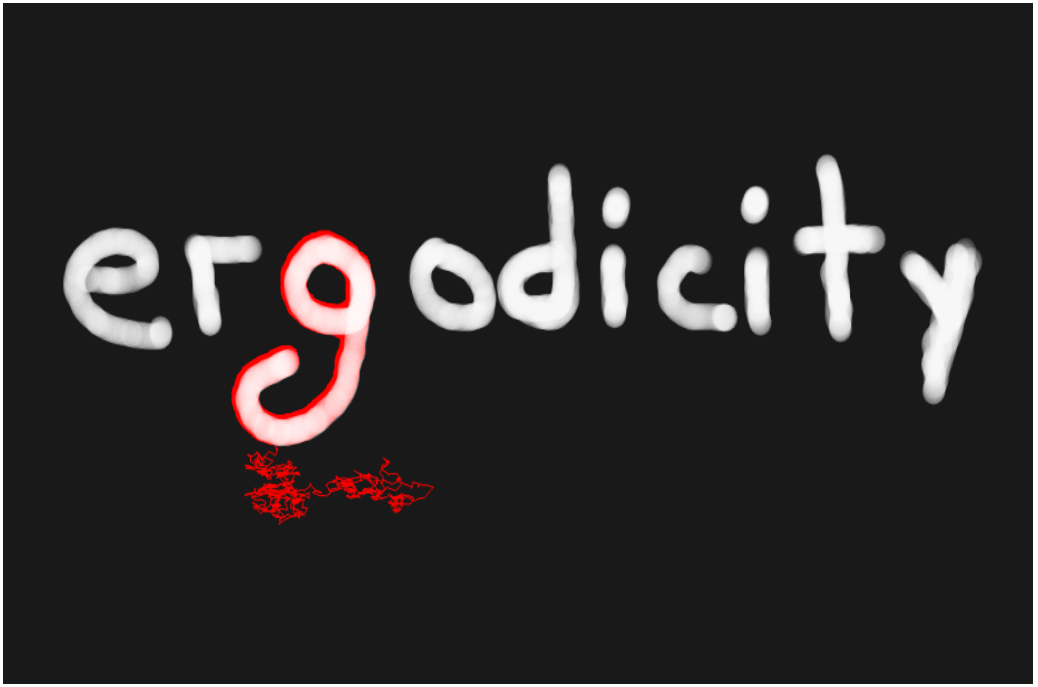
\includegraphics[width=\textwidth]{./images/ergo-4p0.png}
      \caption{$p_\text{big}=0$}
      \label{fig:ergo-subfig-a}
  \end{subfigure}%
  \begin{subfigure}[t]{0.5\textwidth}
      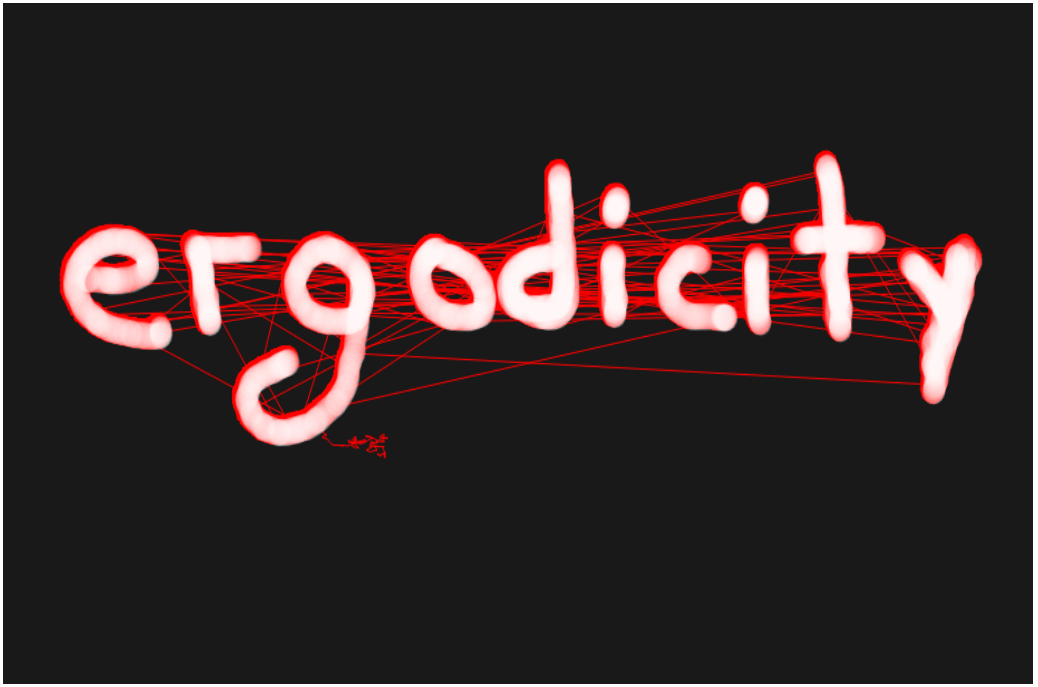
\includegraphics[width=\textwidth]{./images/ergo4p1000.png}
      \caption{$p_\text{big}=10^{-3}$}
      \label{fig:ergo-subfig-b}
  \end{subfigure}
  \caption{A two-dimensional function representing an arbitrary, hand-drawn image is shown, where pixel brighntess corresponds to a function value between zero and one. This function is sampled using $10^6$ samples generated by the Metropolis-Hastings algorithm for two different values of $p_{\text{big}}$ in addition to a Gaussian proposal distribution with $\sigma=4\cdot 10^{-3}$ in normalized image coordinates $[0;1]^2\subset \mathds{R}^2$. The resulting Markov chain of sample positions is connected using a thin red line to visualize the evolution of the Markov chain. For $p_\text{big}=0$, ergodicity is not guaranteed and indeed the Markov chain remains on an island of function values $f(\vek{x})>0$ on the first letter \textit{g} that it encounteres after a transient phase, showing that the stationary distribution that the chain converges to is \textit{not} independent of the initial sample position. For $p_\text{big} = 10^{-3} > 0$, ergodicity is ensured, and global mutations are proposed from a uniform distribution, allowing the chain to 'jump' from one letter to another and correctly sample the entire domain of the function.}
  \label{fig:ergodicity}
\end{figure}


An illustration of the effect of ensuring ergodicity is shown in \autoref{fig:ergodicity}, where a non-zero probability of a global mutation in the proposal distribution leads to the stationary distribution being independent of the initial sample location $x_0$, while a non-ergodic chain may remain stuck on a so-called \textit{island} of points $x$ with $f(x)>0$ that are surrounded by an area of zero contribution that local, small-step mutations such as from a normally distributed proposal distribution around the previous sample are unable to cross. In practice, not just the possibility of a global mutation required to ensure asymptotic correctness, but also the probability thereof can be highly relevant, since the speed of convergence can be highly affected by this parameter \autocite{pbrt}. It is easy to imagine that a higher probability of global mutations might increase the rate of convergence to the stationary distribution if, for example, the function consists of few and small disconnected volumes in the domain with large contributions that cannot be discovered through local mutations of the sample position in $\Omega$ \autocite{pbrt}.

\autoref{fig:ergodicity} also illustrates a concept that is commonly invoked in discussions of Markov chains: recurrence and transience. A recurrent class is a set of positions that are mutually reachable by the Markov chain \autocite{transient-recurrent}, while a transient state (here: $f(x)=0$) will not be reached again under normal circumstances by the Markov chain once visited \autocite{transient-recurrent}, since the acceptance probability $\alpha$ for proposals with zero contribution is zero, unless already at a position with $f(x)=0$. An aperiodic Markov chain with at most one recurrent class, where all points $\left\{ x \in \Omega: f(x)>0\right\}$ with some contribution to the integral of $f$ are mutually reachable, is an ergodic chain \autocite{transient-recurrent}, yielding an alternative interpretation of the requirements for correctness.


In summary, correctness of Metropolis-Hastings can practically be ensured by simply allowing so-called global mutations (proposals drawn uniformly from the state space) with non-zero probability $p_\text{big}$. All other required properties of the Markov chain follow by construction of the algorithm.

\section{Choosing Proposal Distributions}\label{sec:proposal-dist}

Ensuring ergodicity and correct convergence is not the only concern when choosing a proposal distribution. The choice of proposal distribution (also referred to as mutation strategy) determines the rate of convergence, acceptance probability of each proposal and the efficiency of the algorithm as a whole. It is the main degree of freedom of the algorithm to be chosen in accordance with any prior knowledge of the function to be sampled in order to achieve optimal results. Proposal distributions can be classified into families of strategies, two of the most significant of which are random walks and independence chains \autocite{understanding-mh-chib-greenberg}:
\begin{enumerate}
  \item \textbf{Random Walks} have the form $q(x\to x') = q_1\br{\abss{x - x'}}$ and therefore depend only on the distance between current sample $x$ and proposal $x'$ with respect to some metric on the state space \autocite{transience}. This means that $x'$ is drawn as $x' = x + z$ where $z$ is some \textit{increment random variable} determined by $q_1$ \autocite{understanding-mh-chib-greenberg}. Possible distributions $q_1$ include multivariate normal or multivariate Student t-distributions \autocite{bayesian-gibbs-mcmc}.
  \item \textbf{Independence Chains} are, as the name implies, independent of the current sample position $x$ instead of being conditional on them, meaning that they have the form $g(x\to x') = q_2(x')$ \autocite{understanding-mh-chib-greenberg}. Effectively, such a sampling defines a \textit{weighting function} $w(x) = \frac{\pi(x)}{q(x)}$ on the domain, the ratio $\frac{w(x')}{w(x)}$ of which determines the acceptance probability \autocite{bayesian-gibbs-mcmc}, and can therefore be used to implement importance sampling of known features of the target stationary distribution $\pi$, such as when it is of product form where one factor can be sampled and the other is uniformly bounded \autocite{understanding-mh-chib-greenberg}. 
\end{enumerate}

Note that this taxonomy is neither complete nor particularly strict and mutation strategies can be mixed and combined. For example, this report has already mentioned a multivariate normal distribution used to generate small, local mutations resulting in the random walk shown in \autoref{fig:ergo-subfig-a}, as well as how to combine it with a global mutation or uniformly random sampling of $\Omega$ independent of the sample location $x$ to ensure ergodicity, which is by itself an instance of an independence chain, to yield a combined mutation strategy resulting in the Markov chain illustrated in \autoref{fig:ergo-subfig-b}.\\

Not just the class of proposal distribution but also the specific parameters thereof are relevant for optimal convergence. As already mentioned for a Gaussian random walk combined with a uniform global mutation, the choice of the parameter $p_\text{big}$ is relevant to the efficiency since it represents a kind of \textit{exploration-exploitation} trade-off, as is often the case for algorithms that perform any kind of sampling of a state space:

If the chain converges to the correct solution, then samples with higher values of $f(x_k)$ are more commonly visited by the chain, so proposals that are spatially close to a current sample are promising candidates, since they will likely achieve similarly high function values if the underlying function is locally smooth in any sense, which means that local mutations can better exploit this smoothness compared to random guesses and offer a higher acceptance rate and faster speed of convergence. On the other hand, more global mutations can help faster explore a state space consisting for example of many, otherwise mutually unreachable islands of the domain on which $f(x_k)\gg 0$, which are surrounded by volumes with zero contributions where proposals cannot be accepted since $\alpha = 0$, or it could help explore volumes with high function values in a very large state space despite averse initialization at low function values, where finding the more promising volume by random walk would otherwise take extremely many mutations.

A similar argument can be made for other parameters of the proposal distribution, such as the variance $\sigma^2$ for a Gaussian random walk: if the variance is too small, the increments will be small and little progress in terms of convergence to a global solution will be made per iteration \autocite{optimal-mcmc-scaling}. In fact, for a smooth function $f$ and a symmetric proposal distribution, an arbitrarily small perturbation will result in an acceptance rate $\alpha = \frac{f(x')}{f(x_k)}$ that is arbitrarily close to one, due to continuity, but this obviously does not guarantee faster convergence of the Markov chain. 
On the other hand, a variance that is too large could result in an excessively high rate of rejected proposals \autocite{optimal-mcmc-scaling}, which are in a sense a waste of computational resources since they contribute little to the convergence towards the stationary distribution compared to an accepted proposal. Intuitively, accepted proposals can be thought of as providing new information about the target distribution, whereas null steps rather prevent the quality of the current approximation to the target distribution from degrading.\\


There exist theoretical results that show optimal acceptance rates $\chi$ which ensure the most efficiency convergence to the stationary distribution of the Markov chain for various target and proposal distributions in various dimensions. Perhaps the most famous result is that for a Gaussian random walk under relatively weak assumptions, as the dimensionality of the state space $\Omega$ goes to infinity, the asymptotically optimal acceptance rate is $\chi=0.234$ and the variance should be set accordingly, roughly in $\mathcal{O}\br{d^{-1}}$ in the number $d$ of dimensions \autocite{transience}, giving a solid heuristic for tuning of Metropolis-Hastings parameters \autocite{optimal-mcmc-scaling}. Optimal acceptance rates depend on proposal and target distributions and tend to be higher when the number of dimensions is lower \autocite{optimal-low-dim-lower}, where for example the asymptotically optimal acceptance rate of a Gaussian random walk with a Gaussian target distribution in one dimension is $\chi=0.44$ \autocite{optimal-1d-044}. The impact of the probability of global mutations $p_\text{big}$ and the variance $\sigma^2$ of a Gaussian random walk on the convergence and acceptance rate $\chi$ of a Metropolis-sampled Markov chain is illustrated in \autoref{fig:var-pbig}.\\



\begin{figure}
  \centering
  \begin{subfigure}[t]{0.5\textwidth}
      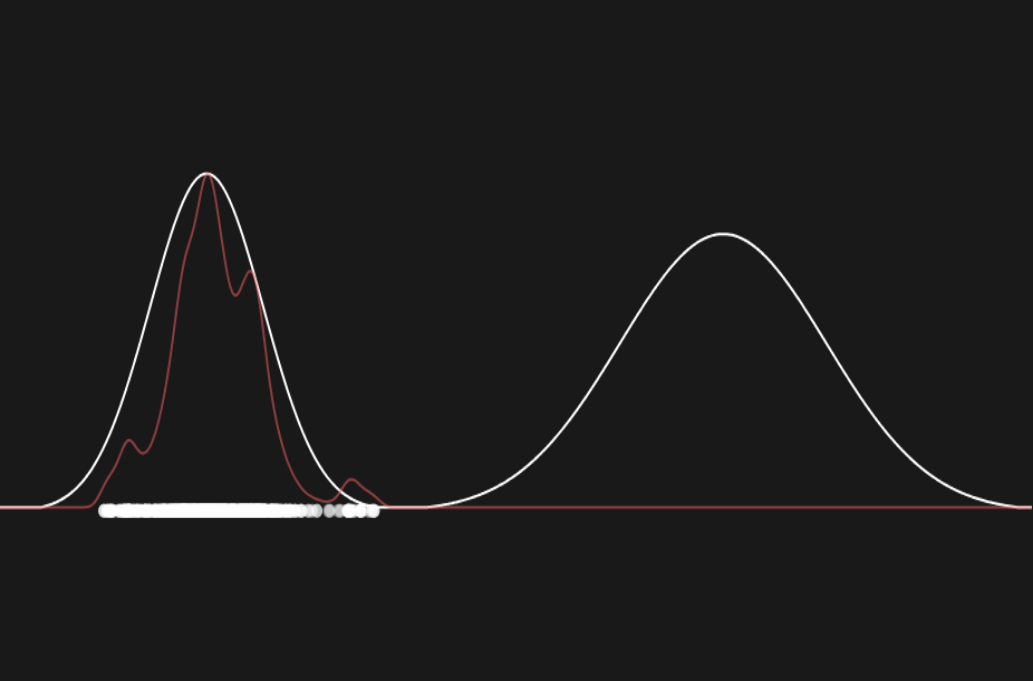
\includegraphics[width=\textwidth]{./images/std1-pbig0-acc94.0-gen41.8.png}
      \caption{$p_\text{big}=0, \sigma^2=0.01 \Longrightarrow \chi = 94.0\%, \epsilon=41.8\%$}
      \label{fig:var-pbig-a}
  \end{subfigure}

  \vspace{0.5cm}

  \begin{subfigure}[t]{0.5\textwidth}
    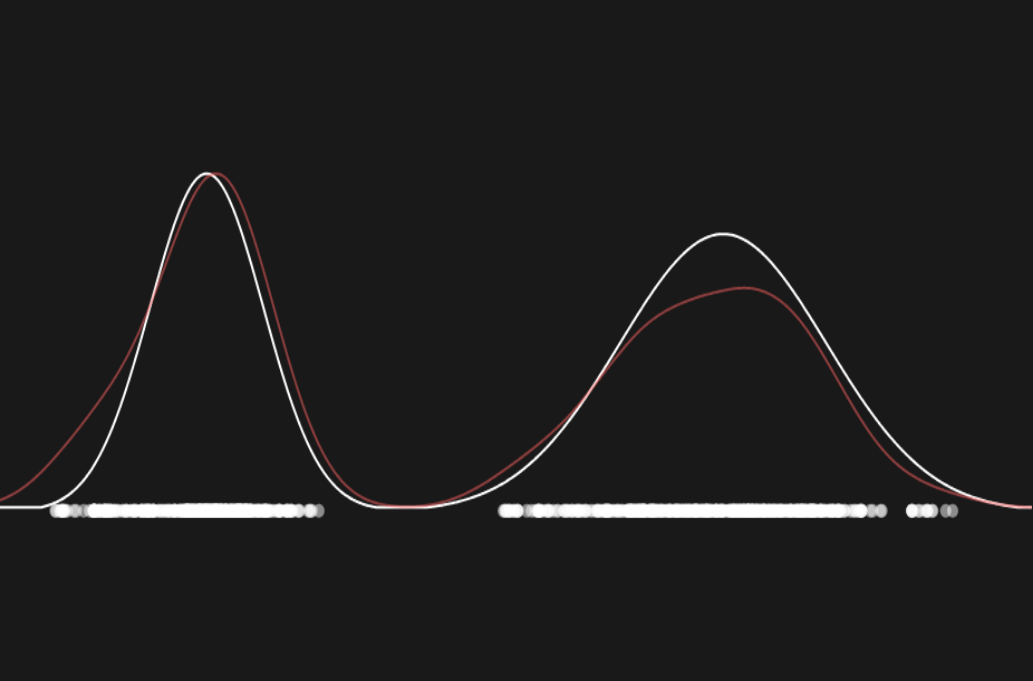
\includegraphics[width=\textwidth]{./images/std1-pb10-acc90.9-gen91.1.png}
    \caption{$p_\text{big}=0.1, \sigma^2=0.01 \Longrightarrow \chi = 90.9\%, \epsilon=91.1\%$}
    \label{fig:var-pbig-b}
  \end{subfigure}

  \vspace{0.5cm}

  \begin{subfigure}[t]{0.5\textwidth}
      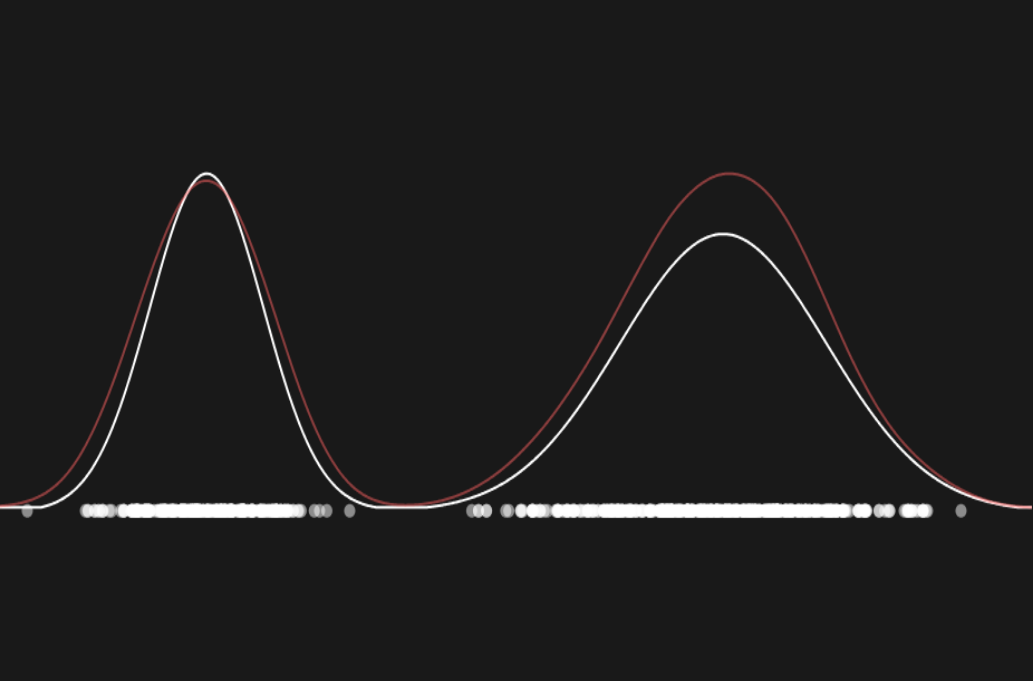
\includegraphics[width=\textwidth]{./images/std20-pb10-acc48.7-gen98.8.png}
      \caption{$p_\text{big}=0.1, \sigma^2=0.2 \Longrightarrow \chi = 48.7\%, \epsilon=98.8\%$}
      \label{fig:var-pbig-c}
  \end{subfigure}
  \caption{The impact of a proposal distribution with different global mutation probabilities $p_\text{big}$ and variances $\sigma^2$ of a Gaussian Random Walk on the Metropolis-Hastings algorithm are illustrated. The function $f$ to be sampled on the domain $[0;1]\subset\mathds{R}$ is shown as a white line, the first $N=1000$ samples of the Markov chain are shown as semi-opaque points along the horizontal axis and a scaled, smoothed reconstruction of the normalized sample density $\langle p \rangle$ using SPH interpolation is shown in red to illustrate the distribution of samples for the three shown realizations of the chain. The accuracy of the sample distribution $\epsilon$ is quantified as the absolute relative error between the analytical integral and a Markov chain Monte-Carlo estimate of the integral using the approximate sample density $\langle p \rangle$ as: $\epsilon = 1 - \frac{\abs{\int_{0}^{1}f(x)\,dx - \frac{1}{N}\sum_{k=1}^{N} \frac{f(x_k)}{\langle p \rangle (x_k)}}}{\abs{\int_{0}^{1}f(x)\,dx}}$. For the chain in \autoref{fig:var-pbig-a} that uses no global mutations and only very small local mutations ($\sigma^2=0.01$) it can be observed that the chain is stuck on the left peak of the function, unable to explore the right peak since local mutations are too small to overcome the gap of zero-contribution values separating the islands. Ergodicity is not achieved in this case, and the result is an incorrect stationary distribution. Since variance is very small and the sampled function is piecewise smooth, proposal function values $f(x')$ and current values $f(x_k)$ are similar and the acceptance rate $\chi$ is extremely high at $94.0\%$, which hints towards slower than necessary convergence to the stationary distribution. Since the stationary distribution is wrong, i.e. not the target distribution, accuracy $\epsilon$ is low. This is remedied in \autoref{fig:var-pbig-b} where global mutations with $p_\text{big}=10\%$ are introduced, ensuring ergodicity and improving the accuracy $\epsilon$, while slightly decreasing the acceptance rate, which is still far above the recommended optimal values for this target distribution that is approximately a multimodal Gaussian target. \autoref{fig:var-pbig-c} shows that by increasing the variance to $\sigma^2=0.2$ and therefore decreasing the acceptance rate of $\chi=48.7$\% closer to guideline values for this one-dimensional problem (See $\chi=44\%$ for \autocite[a 1D Gaussian target using Gaussian random walks]{optimal-1d-044}) a higher accuracy at $\epsilon = 98.8\%$ is achieved and the scaled, smoothed reconstruction of sample densities closely resembles the function $f$.} 
  \label{fig:var-pbig}
\end{figure}

Lastly, note that both the global mutation $\mathcal{U}\br{\Omega}$ and the Gaussian random walk with a multivariate normal distribution are symmetric, so the Hasting-Term becomes one and the acceptance rate simplifies essentially to $\alpha=\frac{f(x')}{f(x_k)}$ as stated in \autoref{eq:alpha-symmetric}.



\section{Benefits and Drawbacks}\label{sec:pros-and-cons}

Metropolis-sampling is not so much a universally applicable sampling strategy as it is a highly effective tool for very specific problems, due to its specific benefits and drawbacks, some of which are briefly outlined in the following.

Some benefits that make the algorithm particularly suited to the application in Computer Graphics include:
\begin{itemize}
  \item \textbf{Few assumptions on $f$ and $\Omega$} There are surprisingly few restrictions on the function $f$ that may be sampled by the Metropolis-Hastings algorithm. In particular, there are no continuity or differentiability constraints and there are very few assumptions on the domain $\Omega$, which need not be real-valued or even continuous. Perhaps most importantly, the normalization constant $b = \int_{\Omega} f(x)\,d\Omega$ need not be known and an arbitrary unnormalized probability density may be used \autocite{survey}. 
  \item \textbf{Flexibility} All that is required of the function $f$ is the ability to evaluate it \autocite{pbrt}. This makes Metropolis-sampling flexible enough to handle rendering tasks, in which abstract path spaces might need to be sampled according to unknown radiance functions that can only be pointwise evaluated and are highly discontinuous due to occlusions. It can sample from a wider variety of functions efficiently compared to rejection sampling for example, the computational cost of which for the generation of a subsequent sample cannot be bounded for many practically relevant functions \autocite{pbrt}.
  \item \textbf{Importance Sampling and Quadrature of Product Forms} In particular, Metropolis sampling is very well-suited to perform \textit{importance sampling} in Monte-Carlo integration, where samples generated from a distribution similar to the integrand (and ideally proportional to it) greatly decrease the variance of the estimator of an integral. Metropolis-Hastings allows precisely such a sampling proportional to a given function with an unknown normalization constant. This makes the Metropolis-Hastings algorithm a great choice for quadrature of integrals of product form $\int_\Omega f(x)h(x) \,d\Omega$ where $f$ is non-negative and $h$ is arbitrary, since if samples are drawn $x_k \sim p$ with $p\propto f$ then the estimator simplifies to $\int_\Omega f(x)h(x) \,d\Omega \overset{\text{MC}}{\approx} \frac{1}{N}\sum_{k=1}^{N} \frac{h(x_k)f(x_k)}{p(x_k)} \overset{\text{MH}}{\approx} \frac{b}{N} \sum_{k=1}^{N} h(x_k)$ \autocite{survey}. While the samples generated by the Markov Chain themselves cannot be used to estimate $b$ \autocite{survey}, this is still very useful if many such integrals (e.g. one per pixel) must be calculated that all share a common normalization constant $b$, as will be abused in the PSSMLT method in \autoref{sec:pssmlt} \autocite{survey}.
  \item \textbf{Specialized Mutation Strategies} Due to the degree of freedom of the Metropolis-Hastings algorithm being not just some scalar parameters but an entire proposal distribution on the state space, there exist uncountable ways to incorporate prior knowledge and assumptions about the function to be sampled into specialized mutation strategies that provide more efficient exploration of the state space, including the ability to dynamically mix highly specialized and more general and robust mutation strategies. Veach and Guibas highlight this in their paper on the original \autocite[Metropolis Light Transport algorithm]{veach-guibas-mlt}, where bidirectional mutations as well as lens and caustic perturbations and multi-chain perturbations are described that can efficiently explore otherwise extremely hard-to-sample parts of the path space in a rendering problem well, resulting in a more robust light transport simulation \autocite{veach-guibas-mlt}.
\end{itemize}

On the other hand, drawbacks and some of their possible fixes include:
\begin{itemize}
  \item \textbf{Startup Bias} The invariance of the Markov chain implied by detailed balance ensures by construction that if a current sample $x_k$ follows the target stationary distribution $\pi$, then the subsequent sample $x_{k+1}$ generated by the Markov chain is also distributed according to $\pi$. However, while the Markov chain converges to the stationary distribution, it only reaches it at infinity \autocite{survey}. For a low number of samples in particular, the distribution of the samples can be far from the stationary distribution, leading to the problem of \textit{startup bias} \autocite{pbrt}. The simplest remedy would be to simply discard some initial number of samples, referred to as the \textit{burn-in period} \autocite{burn-in}, but unfortunately this is neither efficient nor can the number of samples that should be discarded be easily estimated \autocite{survey}. There exist methods to more efficiently eliminate startup bias, in particular due to Veach and Guibas \autocites{veach-guibas-mlt}{survey}, which construct a discrete distribution to draw from $\pi$-likely candidate initial samples obtained in the process of Monte-Carlo estimating the normalization constant $b$ using some other sampling scheme, and where that estimate of $b$ is finally used as the normalization constant for the Markov chain \autocite{survey}.
  \item \textbf{Sample Correlation} Especially when local mutations in some sense of locality on $\Omega$ are used, it is apparent that subsequent samples in the Markov chain are correlated \autocite{bayesian-gibbs-mcmc}. Unfortunately, this correlation can increase the variance and error of a Monte-Carlo estimator that uses the samples $x_k$ generated by the Markov chain for quadrature \autocite{pssmlt}. Correlation can be decreased by discarding all but every $n$-th sample for some $n$ or by observing the realizations of multiple, independent Markov chains \autocite{bayesian-gibbs-mcmc}. For reasons of computational efficiency, discarding samples does not seem to be popular in most applications to image synthesis in Computer Graphics.
  \item \textbf{Transience} If the Metropolis-Hastings algorithm is initialized at $x_0$ where $f(x_0)=0$ then there might be a sequence of transient states are visited, the proposal of which would have been rejected from any $x_0$ for which $f(x_0)>0$ \autocite{transient-recurrent}. These samples should have zero contribution to the desired distribution of samples and should be discarded. This is related to but not the same as the more generally used term \textit{transient phase}, which is used to refer to any initial distribution of samples generated by the Markov chain which is unrepresentative of the desired distribution, with the \textit{startup bias} discussed previously being one such symptom \autocite{burn-in}.
  \item \textbf{Uncertain Convergence} Similar to the issue of startup bias, it is hard to know when a given Markov chain has 'sufficiently' converged. Common workarounds in application to Monte-Carlo integration include running independent Markov chains in parallel and comparing the resulting estimators, stopping when they agree on a value \autocites{veach-guibas-mlt}{survey}. This unfortunately does not guarantee that all chains have adequately explored the entire state space \autocite{survey}.
\end{itemize}




\section{Application: PSSMLT}\label{sec:pssmlt}


\begin{figure}
  
\includegraphics[width=\textwidth]{images/ajar.png}
  \caption{A classic scene introduced in the original \autocite[Metropolis Light Transport paper]{veach-guibas-mlt} that can profit from Metropolis sampling of the path space is shown, rendered by \autocite[Benedikt Bitterli]{ajar}. The entire scene is illuminated only through the slightly ajar door. It is therefore relatively unlikely to find a light-carrying path by random sampling of the path space that actually connects the camera to a light source. Once such a path has been found however, it is very likely that by applying a small mutation to it, such as slightly altering the angle of subsequent line segments along each vertex of the path, a similar path that also leads through the door and into the light can be found. In other words, there are a few continuous islands of volumes with non-zero contribution in a large state space that are surrounded by a fast empty space of zero contribution. This makes local mutations of the path as performed by Metropolis-Hastings that importance-sample the space of paths globally wildly more effective at exploring the integration domain than only using local importance sampling (e.g. of directions in each hemisphere around a path vertex).}
  \label{fig:ajar}
\end{figure}


In the following, an application of the Metropolis-Hastings algorithm to rendering in the form of a Markov chain Monte Carlo algorithm (or MCMC for short) will be outlined using the example of the so-called \textbf{Primary Sample Space Metropolis Light Transport} or PSSMLT method due to \autocite[Kelemen, Szirmay-Kalos, Antal and Csonka (2002)]{pssmlt}. The general idea in Metropolis Light Transport is to use Metropolis sampling as a method for importance-sampling the integrand in a Monte Carlo estimator of an integral which has a product form, as briefly discussed in \autoref{sec:pros-and-cons}. PSSMLT is a special case of this, which uses the \textit{primary sample space} as a state space $\Omega$ to run a Markov chain on, which is the space of random numbers from zero to one $\Omega = [0;1]^d$ for some dimension $d$ that is used by some stochastic raytracer to sample the radiance arriving at a sensor element from an illuminated scene, for example by picking a new direction in a hemisphere to continue a path in or by choosing a random value in Russian Roulette for path termination \autocite{pssmlt}. This allows the PSSMLT method to integrate seamlessly with any existing implementations of stochastic raytracers, be they uni- or bidirectional, on top of any local importance sampling of the path space inherent to the raytracer such as light source and BRDF-sampling \autocite{pssmlt}, Next Event Estimation or the combination of all of these techniques using multiple importance sampling and so on. An example of a scene that can profit from Metropolis-sampling of the path space on top of local importance sampling is shown in \autoref{fig:ajar}.\\

One core insight behind using the primary sample space as the state space instead of directly manipulating the geometry of a light-carrying path (as done in Veach-style Metropolis Light Transport \autocite{veach-guibas-mlt}), is the idea that any stochastic raytracer can be seen as a function from the primary sample space to a non-negative radiance value:
\begin{align*}
  L: [0;1]^d \to \mathds{R}^+\\
   \vek{x} \mapsto L(\vek{x})
\end{align*}
where $\vek{x}$ is a vector in the primary sample space. This mapping can be constructed by letting the first two components of $\vek{x}$ be the normalized coordinates $x_c, y_c$ of the position of the incident radiance on the sensor for some camera model, which (with additional components required for camera models more complex than a pinhole) uniquely determines the initial segment of some straight-lined path from the sensor element into the scene \autocite{pbrt}. Even tough a stochastic raytracer is used, it relies on a random number generator in implementation, meaning that it can also be implemented as a deterministic function on some vector of random numbers. This means that for a given $\vek{x}$, not just the initial segment but an entire path (or multiple paths) through the scene can be uniquely defined and the radiance function $L$ can be sampled \autocite{pbrt}. Furthermore, the maximum number of random numbers $d$ required by any single evaluation of $L$ can be bounded in practice, either a-priori by terminating paths that exceed a certain length (which might introduce bias) or by observing the random number count required during rendering and increasing the upper bound of the dimensionality of the primary sample space $d$ on demand \autocite{pbrt}. Either way, we obtain a simple, convenient, euclidean, unit hypercube $\Omega$ and a mapping from that space to incident radiances to the camera at some position on the image plane.

\begin{highlightblock}
Crucially, note that any implementation of local importance sampling of the radiance function inside the implementation of the raytracer that defines $L$ has the effect of making a greater fraction of random paths form a brighter connection between the camera and a light source in expectation. In other words, any importance sampling in the raytracer has the effect of increasing the volume in the primary sample space that is taken up by brighter paths as compared to lower-contribution paths. This means that even a simple, symmetric local mutation on the primary sample space with a fixed size will result in an implicit importance sampling of the path space with respect to some scalar measure of the (possibly spectrally-valued) radiance, e.g. its luminance \autocite{pssmlt}. In other words, a perturbation of constant size in the primary sample space will result in a larger mutation in the path space where the integrand is small and a smaller mutation where the integrand is large, which is desirable \autocite{pssmlt}. This means that the more sophisticated a raytracer is used in conjunction with PSSMLT, the flatter the integrand becomes in the primary sample space \autocite{mlt-auto-param}, and the greater the synergy between Metropolis sampling on a path-level and other forms of importance sampling on a local level (at each vertex) will become. Apart from the flexibility and convenience of the PSSMLT formalism, this is the core idea behind why this method is effective.
\end{highlightblock}

To derive the concrete method, first note that the intensity of some pixel $I_{x_c,y_c}$ can be written as an integral in product form of the non-negative radiance $L$ and some reconstruction filter $h_{x_c,y_c}$, which in the simplest case might be a rectangular indicator function of normalized sensor positions $\vek{x}_{k, 1}, \vek{x}_{k, 2}$ contributing to pixel $x,y$. This can be approximated using a standard Monte-Carlo sum with samples $x_k \sim p$ as \autocite{pbrt}:
\begin{align}
  I_{x_c,y_c} &= \int_{\Omega} h_{x_c,y_c}(\vek{x}) L(\vek{x}) \, d\Omega &\text{Incoming radiance at pixel location $x,y$}\\
  &\approx \frac{1}{N}\sum_{k=1}^{N} \frac{h_{x_c,y_c}(\vek{x}_k) L(\vek{x}_k)}{p(\vek{x}_k)} &\text{Monte-Carlo estimator}
\end{align}

Using the Metropolis-Hastings algorithm one can construct a Markov chain that samples $\vek{x}_k \sim p$ for a $p \propto I$ where $I(\vek{x})$ is some scalar measure of the intensity of the spectrally-valued radiance $L\br{\vek{x}}$, such as the luminance of $L(\vek{x})$ \autocite{pbrt}. This results in \autocite{pbrt}:
\begin{align}
  I_{x_c,y_c} &\approx \frac{1}{N}\sum_{k=1}^{N} \frac{h_{x_c,y_c}(\vek{x}_k) L(\vek{x}_k)}{p(\vek{x}_k)}
  &\text{Monte-Carlo estimator}\\
  &\approx \frac{1}{N}\sum_{k=1}^{N} \frac{h_{x_c,y_c}(\vek{x}_k) L(\vek{x}_k)}{I(\vek{x}_k)} \underbrace{\br{\int_\Omega I(\vek{x}) \, d\Omega}}_{b :=}
  &\text{Markov chain with $p\br{\vek{x}}\approx\frac{I(\vek{x})}{\int_\Omega I(\vek{x}) \, d\Omega}$}
\end{align}

which means that the image can be generated using a Metropolis-Hastings Markov chain running over the image plane and the primary sample space and for each generated sample simply adding \autocite{pbrt}:
\begin{equation}\label{eq:pssmlt-contribution}
  \frac{b}{N} \frac{h_{x_c,y_c}(\vek{x}_k) L(\vek{x}_k)}{I(\vek{x}_k)} 
\end{equation}
to pixel locations that $\vek{x}_{k, 1} = x_c$, $\vek{x}_{k, 2} = y_c$ contribute to. This also means that the Markov chain will eventually allocate a greater fraction of some given computation budget to brighter areas of the image plane \autocite{pbrt}, which is generally desirable (unless the captured dynamic range is excessively large).

The Markov chain can simply be implemented as a Gaussian random walk where a local mutation $\vek{x}' = \vek{x}_k + \vek{z}$ is defined using multivariate normally distributed noise $\vek{z}\sim\mathcal{N}\br{\vek{\mu} = \vek{0}, \vek{\sigma}}$ of some variance $\vek{\sigma}$ and combined with a global mutation that is applied with some probability $p_\text{big} \in (0;1)$ and which replaces every component of the state vector with a new uniformly random value between zero and one, i.e. $\vek{x}'=\begin{bmatrix}\xi_1 & \xi_2 & \dots & \xi_d\end{bmatrix}^T$ for $\forall i \in \mathds{N}_1^d: \xi_i \sim \mathcal{U}\br{[0;1]}$ \autocite{pbrt}. There exist heuristics for choosing a value of $p_\text{big}$ that ensures an efficient exploration-exploitation trade-off \autocite{mlt-auto-param}. Note that if proposals are periodically wrapped to lie in $[0;1]\subset \mathds{R}$ then both of these mutation strategies, and therefore also the combined proposal distribution, are symmetric, so the Hastings-term in \autoref{eq:alpha-computational} simplifies to one and the simplified acceptance probability from \autoref{eq:alpha-symmetric} may be used in the Metropolis-Hastings algorithm as seen in Alg. \ref{alg:metropolis} to generate all samples. An illustrative example run of the PSSMLT algorithm as outlined here on a simple scalar radiance function using a unidirectional pathtracer with cosine-weighted local importance sampling is shown in \autoref{fig:pssmlt-example}.


\begin{figure}
  \centering
  \begin{subfigure}[t]{0.47\textwidth}
      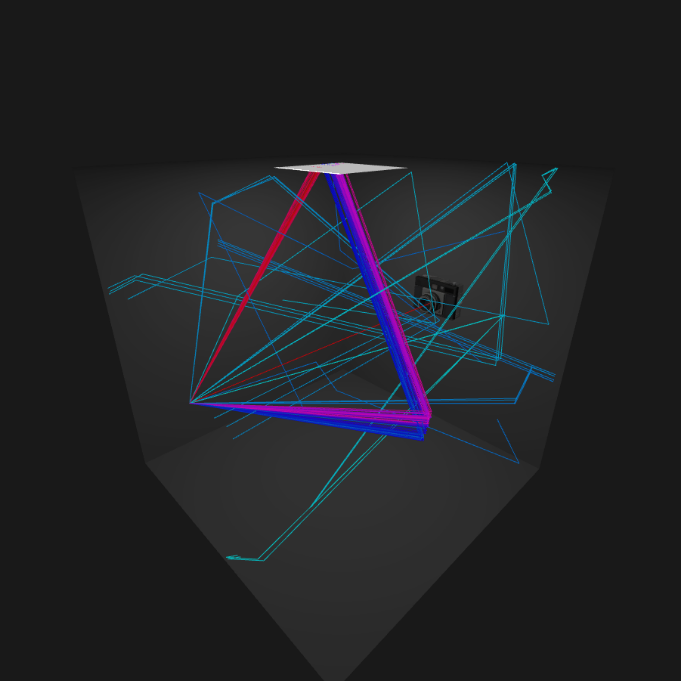
\includegraphics[width=\textwidth]{./images/camview-front.png}
      \caption{front-view of the scene}
      \label{fig:pssmlt-a}
  \end{subfigure}%
  \hspace{0.1cm}%
  \begin{subfigure}[t]{0.47\textwidth}
    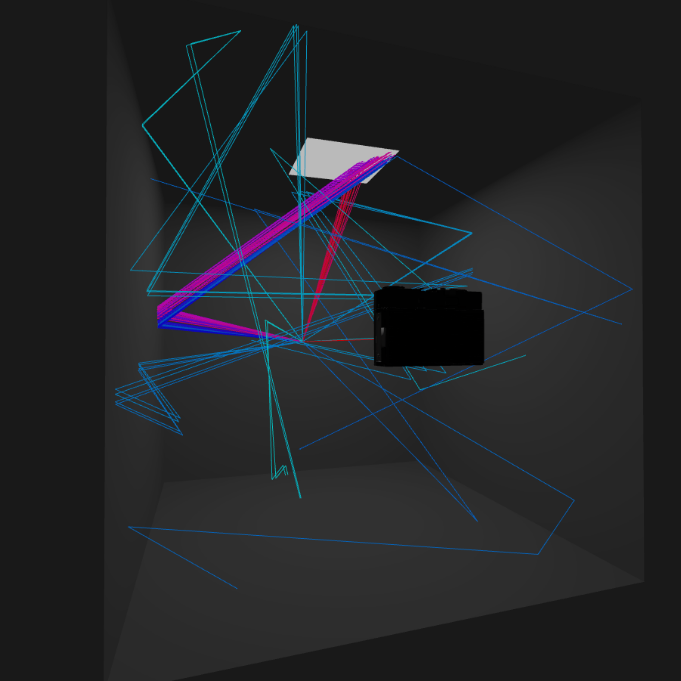
\includegraphics[width=\textwidth]{./images/camview-back.png}
    \caption{back-view of the scene}
    \label{fig:pssmlt-b}
  \end{subfigure}

  \vspace{0.5cm}

  \begin{subfigure}[t]{0.47\textwidth}
    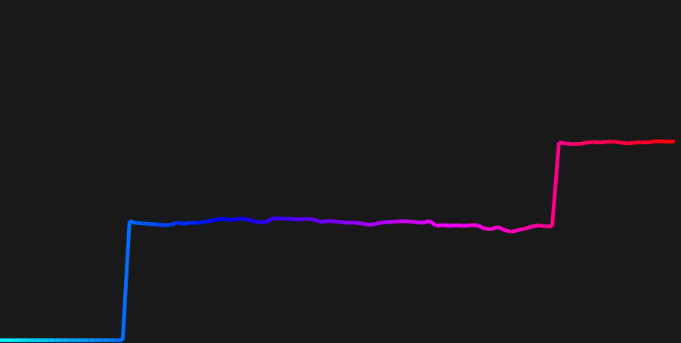
\includegraphics[width=\textwidth]{./images/graphs-l.png}
    \caption{Radiance $L(\vek{x}_k)$ over sample index $k$}
    \label{fig:pssmlt-c}
  \end{subfigure}%
  \hspace{0.1cm}%
  \begin{subfigure}[t]{0.47\textwidth}
    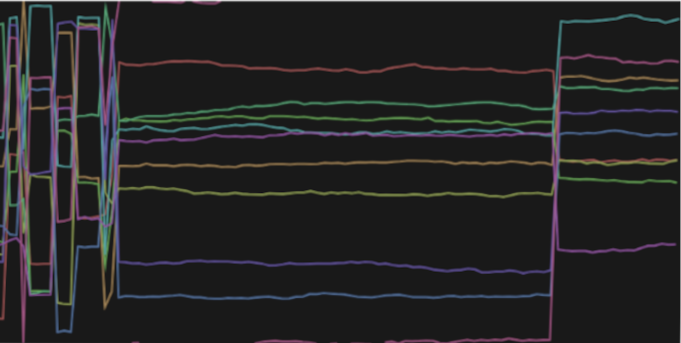
\includegraphics[width=\textwidth]{./images/graphs-pss.png}
    \caption{Components $\vek{x}_{k,1}, \vek{x}_{k,1}, \dots$ of the Primary Sample Space in $[0;1]$ of $\vek{x}_k$ over sample index $k$}
    \label{fig:pssmlt-d}
  \end{subfigure}

  \caption{An example Metropolis sampling of the Primary Sample Space is shown for a box-shaped scene with diffuse walls and a rectangular ceiling light, where a monochrome, scalar-valued radiance $L\br{\vek{x}_k}$ is sampled using a Gaussian random walk with $\sigma_i^2=10^{-3}$ for every dimension $i\in\mathds{N}_1^d$ with $d=10$ and a uniform global mutation with $p_\text{big}=5\%$ for $N=1000$ iterations of the Markov chain. A front and back-view of the scene is illustrated in \autoref{fig:pssmlt-a} and \autoref{fig:pssmlt-b} respectively, which illustrates the pinhole camera position using a 3D model of a camera. Only a single position on the image plane, i.e. a single incident direction to the camera is sampled. Paths are shaded with a hue between blue and red to illustrate the evolution of the sample values for the Markov chain across the $1000$ iterations, with blue paths occurring earlier in the chain than red paths. The corresponding radiances of each sample $L\br{\vek{x}_k}$ over the iteration count $k$ is plotted in \autoref{fig:pssmlt-c} where the $y$-axis is increasing radiance, and each of the corresponding ten components of the sample vector is shown as a different coloured line with the $y$-axis indicating values between zero and one in \autoref{fig:pssmlt-d}. The graphs show an initial phase of transient states visited by the Markov chain as it explores non-light-carrying paths, resulting in zero radiance. During this time, every global mutation is accepted, resulting in regular, uniformly random re-draws of the entire state vector observed in \autoref{fig:pssmlt-d} and resulting, light blue paths in \autoref{fig:pssmlt-a} and \autoref{fig:pssmlt-b} that vary wildly, exploring until finally a three-segment light-carrying path is found. Subsequently, the graphs show small, local mutations which manifest as a group of similar paths exploring the neighbourhood of light-carrying paths in the scene. These paths are illustrated in the scene with a range of blue to magenta colours. During this phase, many global mutations are proposed but not accepted, which is to be expected since the radiance value of most uniformly randomly proposed paths is zero, despite the cosine-weighted BRDF importance sampling of the underlying unidirectional pathtracer. Finally, a global mutation is accepted that results in a ligh-carrying path with only two segments connecting the camera and the light source, resulting in an increased radiance value. After this, a family of similar, high-contribution paths illustrated in the upper images in red is explored.} 
  \label{fig:pssmlt-example}
\end{figure}

\section{Conclusion}
In this report, the Metropolis-Hastings algorithm for creating a Markov chain  of values from a target distribution proportional to some given, non-negative but not necessarily normalized function $f$ was outlined. Sufficient conditions for correct convergence of the Markov chain to the desired, unique stationary distribution were outlined and practical advice on how to guarantee this convergence by ensuring ergodicity of the proposal distribution using so-called global mutations in particular was given. The proposal distribution as the main degree of freedom of the sampling algorithm was investigated and some commonly used classes of mutation strategy along with relevant parameters and their impact and optimality were investigated. Benefits and Drawbacks of Metropolis sampling were discussed, including outlines of mitigation attempts for disadvantages of the method. Finally, the method was practically applied to the context of Markov chain Monte-Carlo rendering in the form of Primary Sample Space Metropolis Light Transport or PPSMLT, including reasoning behind the idea of importance sampling in the path- and state space, a brief derivation, and an illustrative, simple example of a run of PSSMLT.

Metropolis sampling can be concluded to be a helpful tool in rendering especially complex and ill-behaved scenes that would otherwise be extremely difficult to render. This is particularly true for scenes in which only small and few islands of light-carrying paths exist in a vast state space of possible paths that light could take, and where exploring similar paths once a viable one has been found can greatly increase computational efficiency. PSSMLT in particular is useful in scenes where calculating the average luminance of an image is easy, but calculating the distribution of radiances in the image is extremely hard. It is therefore a useful tool in creating especially robust light transport simulations for complex scenes, although it is not without flaws and its advantages for simpler scenes can be brought into question.


\newpage
\printbibliography[
  heading=bibintoc,
  title={Bibliography}
]

\end{document}